%%%%%%%%%%%%%%%%%%%%%%%%%%%%%%%%%%%%%%%%%
% Short Sectioned Assignment LaTeX Template Version 1.0 (5/5/12)
% This template has been downloaded from: http://www.LaTeXTemplates.com
% Original author:  Frits Wenneker (http://www.howtotex.com)
% License: CC BY-NC-SA 3.0 (http://creativecommons.org/licenses/by-nc-sa/3.0/)
%%%%%%%%%%%%%%%%%%%%%%%%%%%%%%%%%%%%%%%%%

%----------------------------------------------------------------------------------------
%	PACKAGES AND OTHER DOCUMENT CONFIGURATIONS
%----------------------------------------------------------------------------------------

\documentclass[paper=a4, fontsize=11pt]{scrartcl} % A4 paper and 11pt font size

% ---- Entrada y salida de texto -----

\usepackage[T1]{fontenc} % Use 8-bit encoding that has 256 glyphs
\usepackage[utf8]{inputenc}
%\usepackage{fourier} % Use the Adobe Utopia font for the document - comment this line to return to the LaTeX default

% ---- Idioma --------

\usepackage[spanish, es-tabla]{babel} % Selecciona el español para palabras introducidas automáticamente, p.ej. "septiembre" en la fecha y especifica que se use la palabra Tabla en vez de Cuadro

% ---- Otros paquetes ----

\usepackage{amsmath,amsfonts,amsthm} % Math packages
%\usepackage{graphics,graphicx, floatrow} %para incluir imágenes y notas en las imágenes
\usepackage{graphics,graphicx, float} %para incluir imágenes y colocarlas

% Para hacer tablas comlejas
%\usepackage{multirow}
%\usepackage{threeparttable}

%\usepackage{sectsty} % Allows customizing section commands
%\allsectionsfont{\centering \normalfont\scshape} % Make all sections centered, the default font and small caps

\usepackage{fancyhdr} % Custom headers and footers
\usepackage{url}
\usepackage[hidelinks]{hyperref}
\pagestyle{fancyplain} % Makes all pages in the document conform to the custom headers and footers
\fancyhead{} % No page header - if you want one, create it in the same way as the footers below
\fancyfoot[L]{} % Empty left footer
\fancyfoot[C]{} % Empty center footer
\fancyfoot[R]{\thepage} % Page numbering for right footer
\renewcommand{\headrulewidth}{0pt} % Remove header underlines
\renewcommand{\footrulewidth}{0pt} % Remove footer underlines
\setlength{\headheight}{13.6pt} % Customize the height of the header

\DeclareOldFontCommand{\rm}{\normalfont\rmfamily}{\mathrm}
\DeclareOldFontCommand{\sf}{\normalfont\sffamily}{\mathsf}
\DeclareOldFontCommand{\tt}{\normalfont\ttfamily}{\mathtt}
\DeclareOldFontCommand{\bf}{\normalfont\bfseries}{\mathbf}
\DeclareOldFontCommand{\it}{\normalfont\itshape}{\mathit}
\DeclareOldFontCommand{\sl}{\normalfont\slshape}{\@nomath\sl}
\DeclareOldFontCommand{\sc}{\normalfont\scshape}{\@nomath\sc}
\DeclareRobustCommand*\cal{\@fontswitch\relax\mathcal}
\DeclareRobustCommand*\mit{\@fontswitch\relax\mathnormal}

\numberwithin{equation}{section} % Number equations within sections (i.e. 1.1, 1.2, 2.1, 2.2 instead of 1, 2, 3, 4)
\numberwithin{figure}{section} % Number figures within sections (i.e. 1.1, 1.2, 2.1, 2.2 instead of 1, 2, 3, 4)
\numberwithin{table}{section} % Number tables within sections (i.e. 1.1, 1.2, 2.1, 2.2 instead of 1, 2, 3, 4)

\setlength\parindent{0pt} % Removes all indentation from paragraphs - comment this line for an assignment with lots of text

\newcommand{\horrule}[1]{\rule{\linewidth}{#1}} % Create horizontal rule command with 1 argument of height




%----------------------------------------------------------------------------------------
%	TÍTULO Y DATOS DEL ALUMNO
%----------------------------------------------------------------------------------------

\title{	
\normalfont \normalsize 
\textsc{{\bf Visión por computador (2016-2017)} \\ Grado en Ingeniería Informática \\ Universidad de Granada} \\ [25pt] % Your university, school and/or department name(s)
\horrule{0.5pt} \\[0.4cm] % Thin top horizontal rule
\huge Memoria Práctica 3 \\ % The assignment title
\horrule{2pt} \\[0.5cm] % Thick bottom horizontal rule
}

\author{Ignacio Martín Requena} % Nombre y apellidos

\date{\normalsize\today} % Incluye la fecha actual

%----------------------------------------------------------------------------------------
% DOCUMENTO
%----------------------------------------------------------------------------------------
\usepackage{graphicx}
\usepackage{listings}
\usepackage{color}
\definecolor{gray97}{gray}{.97}
\definecolor{gray75}{gray}{.75}
\definecolor{gray45}{gray}{.45}
 

\lstset{ frame=Ltb,
     framerule=0pt,
     aboveskip=0.5cm,
     framextopmargin=3pt,
     framexbottommargin=3pt,
     framexleftmargin=0.4cm,
     framesep=0pt,
     rulesep=.4pt,
     backgroundcolor=\color{gray97},
     rulesepcolor=\color{black},
     %
     stringstyle=\ttfamily,
     showstringspaces = false,
     basicstyle=\small\ttfamily,
     commentstyle=\color{gray45},
     keywordstyle=\bfseries,
     %
     numbers=left,
     numbersep=15pt,
     numberstyle=\tiny,
     numberfirstline = false,
     breaklines=true,
   }
 


\lstdefinestyle{consola}
   {basicstyle=\scriptsize\bf\ttfamily,
    backgroundcolor=\color{gray75},
   }
 
\lstdefinestyle{C}
   {language=C,
   }



\begin{document}

\maketitle % Muestra el Título

\newpage %inserta un salto de página

\tableofcontents % para generar el índice de contenidos

\listoffigures

\newpage



%----------------------------------------------------------------------------------------
%	Cuestion 1
%----------------------------------------------------------------------------------------

\section{Estimación de la matriz de una cámara a partir del conjunto de puntos en correspondencias}


\subsection{Generar la matriz de una cámara finita P a partir de valores aleatorios en [0,1] . Verificar si representa una cámara finita y en ese caso quedársela.}

Para este primer apartado  se ha implementado la función GenerarMatrizP(Mat \&P) la cual genera una matriz de cámara finita P a partir de valores aleatorios.\\

Para ello en primer lugar generamos 12 numeros aleatorios que son los que compondran la matriz P 3x4 . Como P se puede descomponer como el resultado de [M | m], teniendo entonces M dimensiones 3x3, podemos comprobar directamente si el determinante de  M es mayor que 0 y, en caso de que lo sea, P será una matriz válida.

\subsection{ Suponer un patrón de puntos del mundo 3D compuesto por el conjunto de puntos con coordenadas {(0,x1,x2) y (x2,x1,0), para x1=0.1:0.1:1 y x2=0.1:0.1:1}. Esto supone una rejilla de puntos en dos planos distintos ortogonales}

La función implementada para realizar este segundo apartado es  vector <Point3d>\\  GenerarPatron3D(), la cual devuelve un patrón 3D generado.\\

Esta función lo que hace es  generar los puntos p1= (0,x1,x2) y p2 = (x2,x1,0) siendo x1 y x2 valores que aumentan de 0,1 en 0,1 hasta llegar a 1. De esta forma crearemos 200 puntos.

\subsection{Proyectar el conjunto de puntos del mundo con la cámara simulada y obtener las coordenadas píxel de su proyección.}

Para empezar  realizaremos tres tareas: transformar los puntos 3D del apartado anterior en matrices 4x1, generar los puntos proyectados y generar las coordenadas pixel  usando los puntos proyectados.\\

La primera de estas tareas la realiza la función vector<Mat>generarMatricesDePuntos\\(vector<Point3d> punt) la cual recibe un vector de puntos 3D y crea para cada punto 3D del vector una matriz de 4x1 de la forma: [p[i].x,p[i].y,p[i].z,1].\\

Ahora necesitamos generar los puntos proyectados, de esto se encarga la función  vector<Mat> generarPuntosProyectados(Mat P, vector<Mat> mat) cuya labor es multiplicar la matriz  p  generada en el primer apartado y los puntos 3D transformados en matrices 4x1, lo que devolverá puntos 3D.\\

Acabamos generando las coordenadas pixel. Estas son el resultado de dividir cada coordenada X e Y  de un punto por su correspondiente componente Z en cada uno de los puntos del vector obtenido en el apartado anterior. Lo que obtendremos, por tanto, será un vector  de matrices de dimensiones 2x1.\\


	
\subsection{Implementar el algoritmo DLT para estimar la cámara P a partir de los puntos 3D y sus proyecciones en la imagen.}

Este algoritmo lo vamos a dividir en tres pasos:

\begin{itemize}
	\item \textbf{Calculo de K y R a partir de M}
	
	A partir de la matriz original P y sabiendo que esta es la composición de P=[M|m] calculamos las matrices R y K. Esta tarea la realiza la función calcularRotaciones(M,K,R). Para la implementación de esta función se ha seguido lo expuesto en el apartado de Descomposición de P del tema \textit{Computer Vision: Cameras} explicado en clase, concretamente las diapositivas 45 y 46.\\
	
	Básicamente lo que hacemos es generar las matrices Qx,Qy y Qz, a partir de  calculando c y s a partir de M para Qx, a partir de M*Qx para Qy y a partir de M*Qx*Qy para Qz. Obtenido esto podemos determinar K como M*Qx*Qy*Qz y  R como la transpuesta de Qx*Qy*Qz.\\
	
	
	\item \textbf{Calculo de T}
	
	Una vez obtenida la matriz K, T la deducimos como K$^{-1}$*m
	
	\item \textbf{Obtención de P a partir de K, R y T}
	
	Para ello construimos una matriz 3x4  de la siguiente forma (función obtenerP(K, R, T);):
	
	\[P = K* \left( \begin{array}{cccc}
	r11 & r21 & r31 & t11\\
	r12 & r22 & r32 & t21\\
	r13 & r23 & r33 & t31\end{array} \right)\] 
	
\end{itemize}
	
\subsection{Calcular el error de la estimación usando la norma de Frobenius (cuadrática)}

Para  el cálculo de este error aplicamos la fórmula:

\[
\sum_{i=1}^{n}\sum_{j=1}^{n}(P{ij}-PP_{ij})^{2}
\]

Obteniendo la siguiente salida:

\begin{figure}[H]
\centering
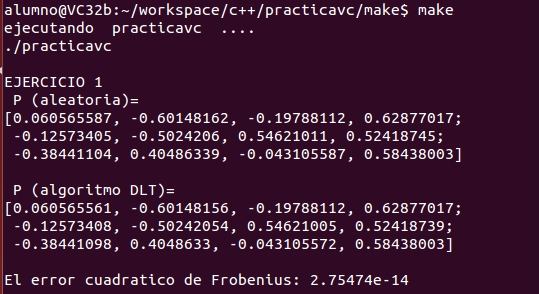
\includegraphics[width=0.7\linewidth]{salida-ej1}
\caption{Salida error Frobenius}
\label{fig:salida-ej1}
\end{figure}

Como podemos ver el error de la estimación usando Frobenius es bastante bajo, por lo que aparentemente podemos afirmar que los resultados son buenos.


%----------------------------------------------------------------------------------------
%	Cuestion 2
%----------------------------------------------------------------------------------------

\section{Calibración de la cámara usando homografías }

\subsection{Escribir una función que sea capaz de ir leyendo las sucesivas imágenes en chessboard.rar y determine cuáles son válidas para calibrar una cámara. Usar las 25 imágenes tiff que se incluyen en el fichero datos. Usar la función cv::findChessboardCorners(). Determinar valores precisos de las coordenadas de las esquinas presentes en las imágenes seleccionadas usando cv::cornerSubpix(). Pintar sobre la imagen los puntos estimados usando la función cv::drawChessboardCorners() ( ver código de ayuda en la documentación de OpenCV)}

Después de la lectura de las imagenes chessboard vamos a ir recorriendolas una a una para determinar si una imagen es o no valida para calibrar una camara, para ello en primer lugar transformamos la imagen a una con escala de grises y, seguidamente, aplicamos la función findChessboardCorners de la siguiente forma:\\

\begin{lstlisting}[language=C]
bool found = findChessboardCorners(gray_image, board_sz, corners, CALIB_CB_ADAPTIVE_THRESH + CALIB_CB_NORMALIZE_IMAGE + CALIB_CB_FAST_CHECK);
if (found) {
	devol = true;
	//Obtenemos los corners
	cornerSubPix(gray_image, corners, Size(11, 11), Size(-1, -1), TermCriteria(CV_TERMCRIT_EPS + CV_TERMCRIT_ITER, 30, 0.1));
	//Dibujamos sobre la imagen
	drawChessboardCorners(gray_image, board_sz, corners, found);
	sal.push_back(gray_image);
}
\end{lstlisting}

Como podemos ver, la funcion findChessboardCorners recibe  la imagen del tablero, el tamaño de este (en nuestro caso 13x12), el vector donde se almacenen las esquinas encontradas y una serie de flags para usar un thresholding adaptativo, normalizar el gamma de la imagen antes de aplicar el thresholding y hacer un checkeo rápido buscando corners para acabar de forma rápida si la imagen no nos sirve.\\

Por último solamente quedaría que, en caso de que la imagen si nos valga, obtener los corners en concreto y dibujarlos sobre la imagen\\

En la salida vamos a obtener que 4 de las 25 imágenes son válidas para calibrar la cámara, en concreto las imágenes numero 9, 11, 17 y 20. Estas imágenes con sus detecciones de esquinas son:

\begin{figure}[H]
	\centering
	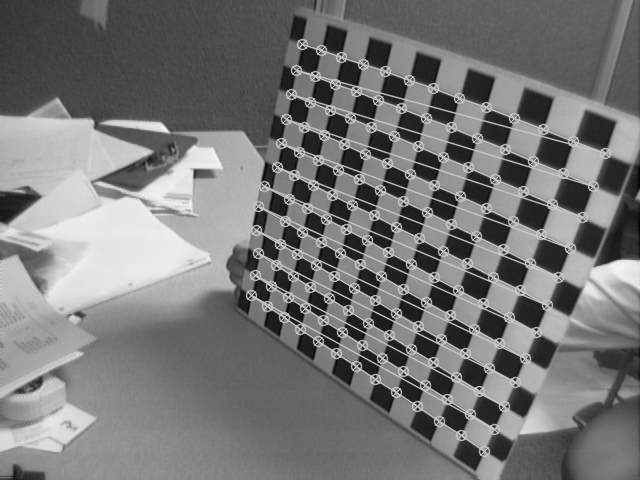
\includegraphics[width=0.7\linewidth]{ej2-1}
	\caption{Detección imagen 9}
\end{figure}

\begin{figure}[H]
	\centering
	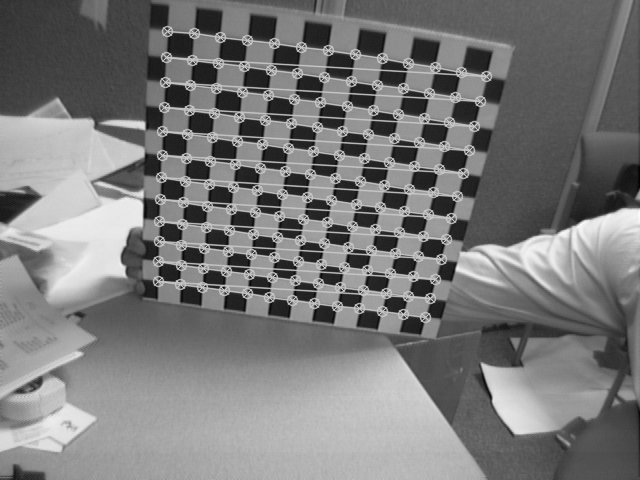
\includegraphics[width=0.7\linewidth]{ej2-2}
	\caption{Detección imagen 11}
\end{figure}

\begin{figure}[H]
	\centering
	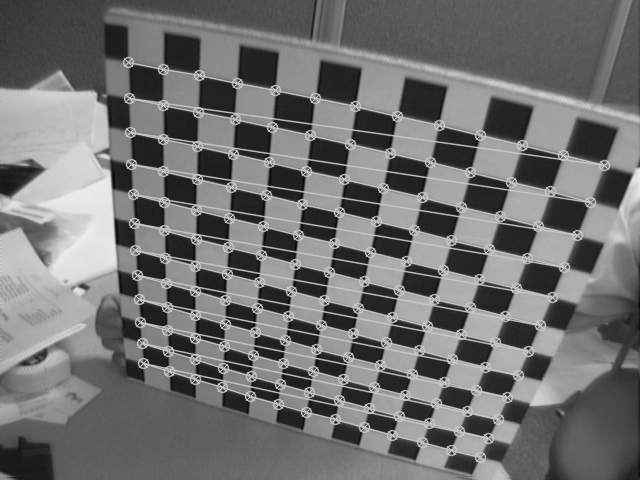
\includegraphics[width=0.7\linewidth]{ej2-3}
	\caption{Detección imagen 17}
\end{figure}

\begin{figure}[H]
	\centering
	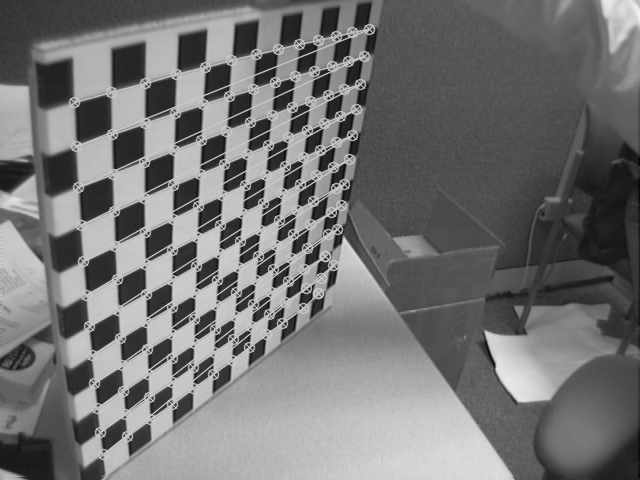
\includegraphics[width=0.7\linewidth]{ej2-4}
	\caption{Detección imagen 20}
\end{figure}


\subsection{Usando las coordenadas de los puntos extraídos en las imágenes seleccionadas del punto anterior, calcular los valores de los parámetros intrínsecos y extrínsecos de la cámara para cada una de dichas imágenes. Usar la función cv::calibrateCamera(). Suponer dos situaciones: a) sin distorsión óptica y b) con distorsión óptica. Valorar la influencia de la distorsión óptica en la calibración y la influencia de la distorsión radial frente a la distorsión tangencial.}

En este apartado el grueso de la cuestión gira en torno a la función de opencv calibrateCamera, la cual se define de la siguiente manera:

\begin{lstlisting}[language=C]
	calibrateCamera(object_points, image_points, image.size(), intrinsic, distCoeffs, rvecs, tvecs, [FLAGS]);
	cout << endl << "distCoeffs con distorsion= " << distCoeffs << endl << endl;
	
	Mat imageUndistorted;
	undistort(image, imageUndistorted, intrinsic, distCoeffs);
	
	cout << endl << "distCoeffs sin distorsion= " << distCoeffs << endl << endl;
	
	sal.push_back(imageUndistorted);
\end{lstlisting}

Obtendremos dos salidas de coeficientes, una con distorsion óptica y otra sin, determinadas por los flags de calibrateCamera (la imagen sin ningun tipo de distorsion se obtiene añadiendo los flags CV\_CALIB\_FIX\_K1 or CV\_CALIB\_FIX\_K2 or CV\_CALIB\_FIX\_K3 or CV\_CALIB\_FIX\_K4 or CV\_CALIB\_FIX\_K5 or CV\_CALIB\_FIX\_K6 or\\ CV\_CALIB\_ZERO\_TANGENT\_DIST).

\begin{figure}[H]
	\centering
	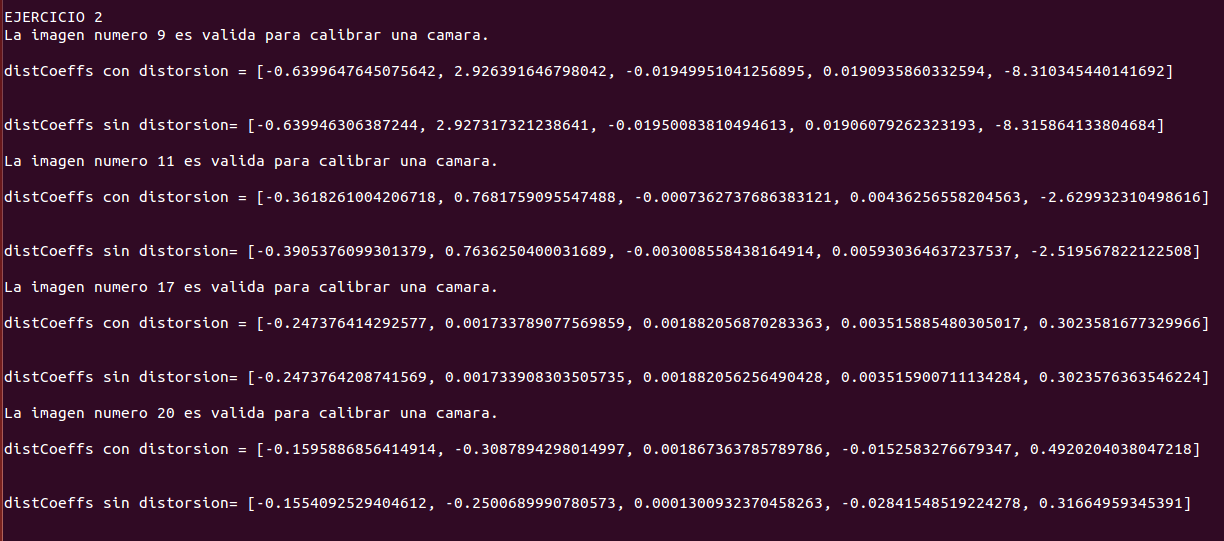
\includegraphics[width=0.9\linewidth]{diffcoefs}
	\caption{Coeficientes con y sin distorsion}
\end{figure}

Como vemos, lo resultados son muy parecidos, por lo que, o a simple vista el hecho de que haya distorsión óptica o no en nuestro caso no influye o quizá la comparación no es la correcta.
%----------------------------------------------------------------------------------------
%	Cuestion 3
%----------------------------------------------------------------------------------------

\section{Estimación de la matriz fundamental F}

\subsection{Obtener puntos en correspondencias sobre las imágenes Vmort[*].pgm de forma automática usando las funciones de BRISK/ORB}

Para este apartado se ha usado parte de la practica anterior. En concreto las funciones de detección de puntos en correspondencia Akaze, kaze y puntosEnComun explicadas en la práctica anterior, por lo que pasaremos directamente a la valoración de los resultados:

\begin{figure}[H]
	\centering
	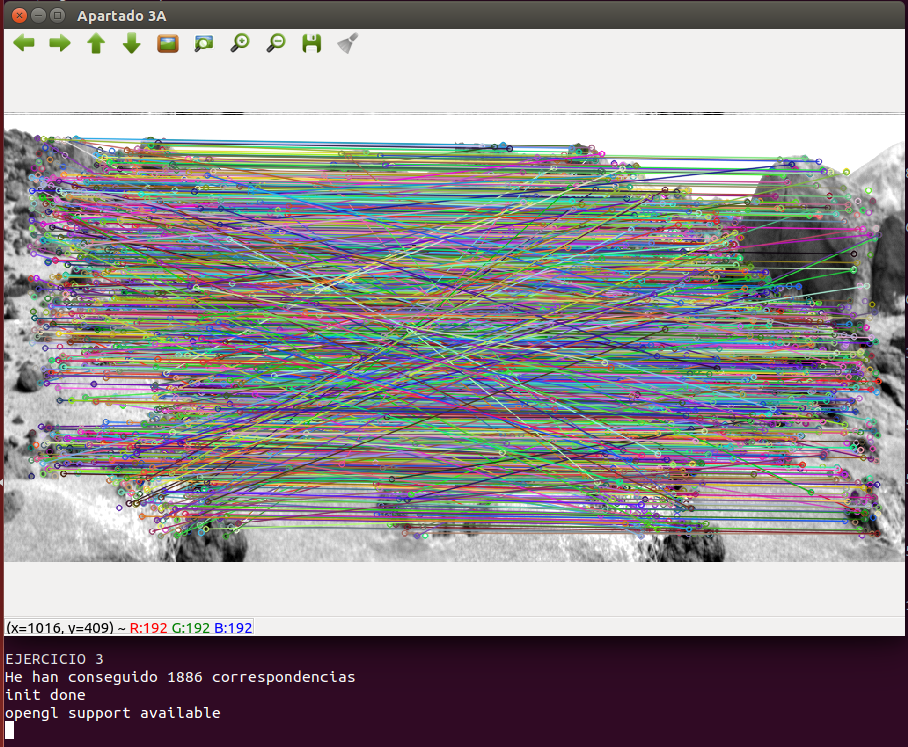
\includegraphics[width=0.9\linewidth]{correspondencia}
	\caption{Correspondencias usando Akaze}
\end{figure}

Hemos obtenido 1886 correspondencias, lo que es un numero bastante elevado.

\subsection{Calcular F por el algoritmo de los 8 puntos + RANSAC (usar un valor pequeño para el error de RANSAC)}

Para este apartado vamos, en primer lugar, a transformar la lista de keypoints que el descriptor Akaze nos proporcionó en el apartado anterior en una lista de Point2f con el objetivo de facilitarnos los cálculos. Una vez hecho esto dibujamos un circulo en la imagen que corresponda en cada punto keypoint anteriormente convertido a Point2f.\\

Una vez hecho esto obtenemos F usando la función findFundamentalMat que proporciona OpenCV y aplica RANSAC de la siguiente forma:

\begin{lstlisting}[language=C]
	F = findFundamentalMat(Mat(points1), Mat(points2), CV_FM_RANSAC, 3, 0.999);
\end{lstlisting}

Obteniendo la matriz F:

\begin{figure}[H]
	\centering
	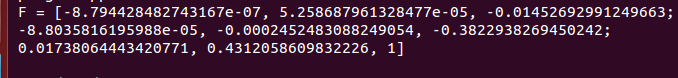
\includegraphics[width=0.9\linewidth]{funcionF3b}
	\caption{Matriz F 3b}
\end{figure}

\subsection{Dibujar las líneas epipolares sobre ambas imágenes ( < 200).}

En primer lugar hacemos uso de la función computeCorrespondEpilines que a partir de los puntos usados en el apartado anterior para generar F y la propia F nos proporciona una lista de parejas de puntos que determinan las lineas obtenidas.\\

Ahora quedaría dibujar las lineas en la imagen y comprobar como de buenos son nuestros resultados. Esto lo hacemos con la función dibujarLineaEpipolar cuyo contenido es:

\begin{lstlisting}[language=C]
Mat dibujarLineaEpipolar(Mat img, vector<Vec3f> lines){
	RNG rng(200);
	Scalar color;
	Mat sal = img;
	uint condfin = 200;
	for (uint i=0; i<condfin; i++){
		color = Scalar(rng.uniform(0, 255), rng.uniform(0, 255), rng.uniform(0, 255));
		line(sal, Point(0, -lines[i][2] / lines[i][1]), Point(img.cols, -(lines[i][2] + lines[i][0] * img.cols) / lines[i][1]), color);
		}
	return sal;
}
\end{lstlisting}

El color de cada linea es determinado aleatoriamente y la posición de cada punto en la imagen se determina directamente en la función line.\\

La salida obtenida en este caso es:

\begin{figure}[H]
	\centering
	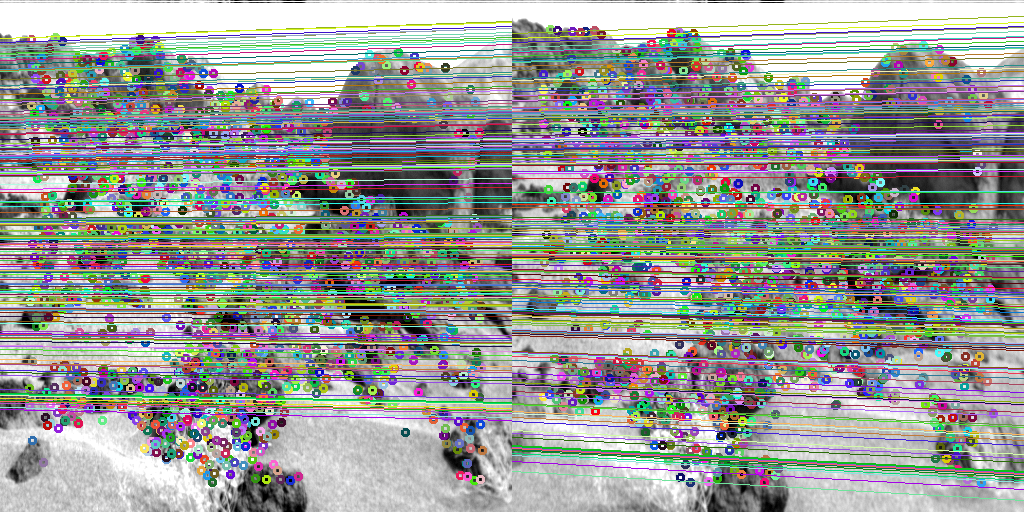
\includegraphics[width=0.9\linewidth]{Apartado-3C}
	\caption{Lineas Epipolares}
\end{figure}

Como podemos observar a simple vista el resultado no es nada bueno, las lineas no siguen ningún patrón esperado. Aquí me ha sido imposible determinar cual es el origen del problema, pero seguramente la raíz de este sea un mal cálculo de la matriz F o un mal cálculo de la posición de las lineas a la hora de pintarlas.


 
\subsection{Verificar la bondad de la F estimada calculando la media de la distancia ortogonal entre los puntos soporte y sus líneas epipolares en ambas imágenes. Mostrar el valor medio del error.}

El calculo del error medio se basa en una media de las distancias entre las lineas y los puntos que hemos obtenido en los apartados anteriores en cada una de las dos imágenes. La bondad obtenida es de 153.146, lo que muestra que los resultados no son muy buenos a priori.

%----------------------------------------------------------------------------------------
%	Cuestion 4
%----------------------------------------------------------------------------------------

\section{Calcular el movimiento de la cámara (R,t) asociado a cada pareja de imágenes calibradas.}

\subsection{Usar las imágenes y datos de calibración dados en el fichero reconstruccion.rar}

En el caso de las imágenes la lectura de estas se ha realizado con funciones de OpenCV como ha sido habitual durante todo el curso. En el caso de los archivos .camera se ha tenido que implementar una función llamada LeerCamera para su lectura. En esta función se ha presupuesto que no existen comentarios en el archivo con el fin de facilitar la programación.

\subsection{Calcular parejas de puntos en correspondencias entre las imágenes }

Este apartado merece poca explicación, ya que lo que vamos a realizar es el calculo de los puntos en común entre las imágenes, cosa que ya hemos implementado en el apartado 3A, por tanto, llamaremos a la función de este apartado y posteriormente convertiremos los keypoints calculados a Point2f con el fin de facilitar los cálculos.

\subsection{Estimar la matriz esencial y calcular el movimiento.}
La estimación de la Matriz esencial la realizamos como hicimos previamente, esto es, usando la función findFundamentalMat la cual nos devuelve una estimación de F.\\

La Matriz de movimiento E sabemos que es el resultado de K2.t()*F*K1, así que podemos calcularla directamente. Tanto la matriz R\_E como la T\_E no he conseguido llegar a ninguna solución razonable.\\

La salida obtenida sería:


\begin{figure}[H]
	\centering
	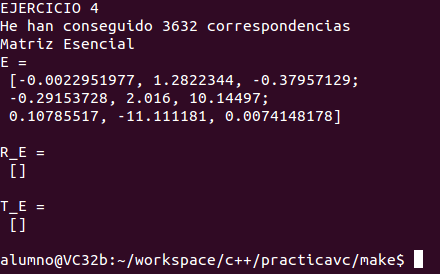
\includegraphics[width=0.9\linewidth]{ej4}
	\caption{Lineas Epipolares}
\end{figure}


\end{document}